\documentclass[border=5mm]{standalone}
\usepackage{tikz}
\usetikzlibrary{shapes.geometric, arrows.meta, positioning, fit}

\begin{document}

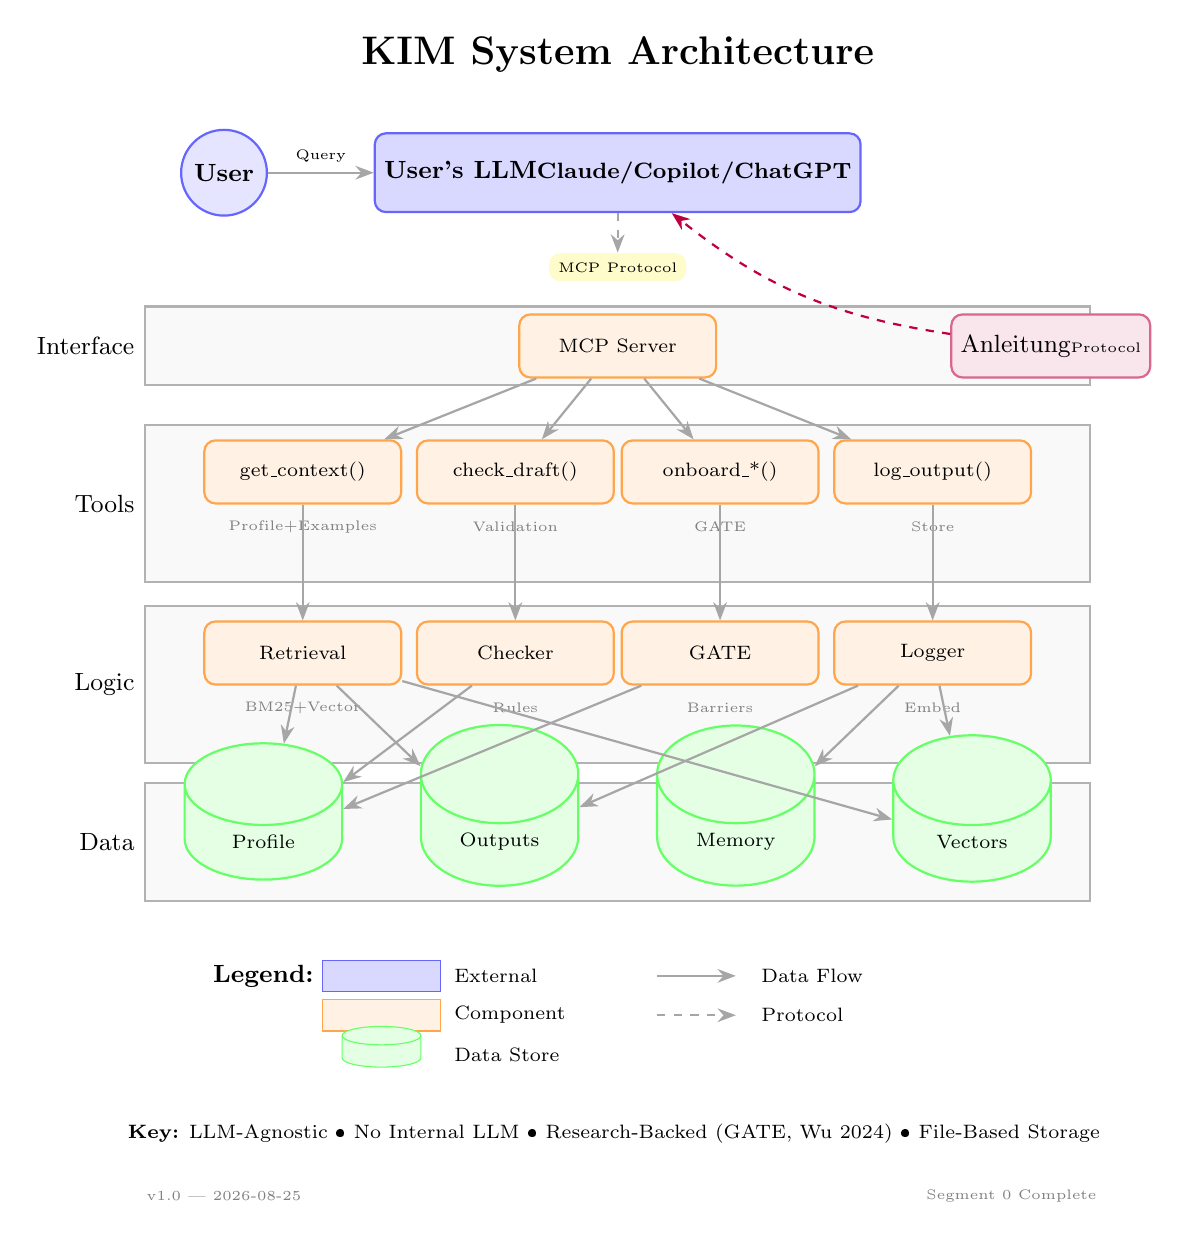
\begin{tikzpicture}[
    node distance=1.2cm,
    actor/.style={circle, draw=blue!60, fill=blue!10, thick, minimum size=1cm, font=\small\bfseries},
    external/.style={rectangle, rounded corners, draw=blue!60, fill=blue!15, thick, minimum width=3.5cm, minimum height=1cm, font=\small\bfseries},
    component/.style={rectangle, rounded corners, draw=orange!70, fill=orange!10, thick, minimum width=2.5cm, minimum height=0.8cm, font=\scriptsize},
    data/.style={cylinder, draw=green!60, fill=green!10, thick, minimum width=2cm, minimum height=0.8cm, shape border rotate=90, font=\scriptsize},
    arrow/.style={-Stealth, thick, draw=gray!70},
    layer/.style={rectangle, draw=gray!60, fill=gray!5, thick}
]

% Title
\node[font=\Large\bfseries] at (0, 9.5) {KIM System Architecture};

% User
\node[actor] (user) at (-5, 8) {User};

% LLM
\node[external] (llm) at (0, 8) {User's LLM\\{\footnotesize Claude/Copilot/ChatGPT}};

\draw[arrow] (user) -- node[above, font=\tiny] {Query} (llm);

% MCP Protocol
\node[font=\tiny, fill=yellow!20, rounded corners] (mcp) at (0, 6.8) {MCP Protocol};
\draw[arrow, dashed] (llm) -- (mcp);

% Interface Layer
\node[layer, minimum width=12cm, minimum height=1cm, label={[font=\small]west:Interface}] (interface) at (0, 5.8) {};
\node[component] (mcp_server) at (0, 5.8) {MCP Server};

% Tools Layer
\node[layer, minimum width=12cm, minimum height=2cm, label={[font=\small]west:Tools}] (tools) at (0, 3.8) {};
\node[component] (t_ctx) at (-4, 4.2) {get\_context()};
\node[component] (t_chk) at (-1.3, 4.2) {check\_draft()};
\node[component] (t_onb) at (1.3, 4.2) {onboard\_*()};
\node[component] (t_log) at (4, 4.2) {log\_output()};

\node[font=\tiny, text=gray] at (-4, 3.5) {Profile+Examples};
\node[font=\tiny, text=gray] at (-1.3, 3.5) {Validation};
\node[font=\tiny, text=gray] at (1.3, 3.5) {GATE};
\node[font=\tiny, text=gray] at (4, 3.5) {Store};

% Logic Layer
\node[layer, minimum width=12cm, minimum height=2cm, label={[font=\small]west:Logic}] (logic) at (0, 1.5) {};
\node[component] (l_ret) at (-4, 1.9) {Retrieval};
\node[component] (l_chk) at (-1.3, 1.9) {Checker};
\node[component] (l_gate) at (1.3, 1.9) {GATE};
\node[component] (l_log) at (4, 1.9) {Logger};

\node[font=\tiny, text=gray] at (-4, 1.2) {BM25+Vector};
\node[font=\tiny, text=gray] at (-1.3, 1.2) {Rules};
\node[font=\tiny, text=gray] at (1.3, 1.2) {Barriers};
\node[font=\tiny, text=gray] at (4, 1.2) {Embed};

% Data Layer
\node[layer, minimum width=12cm, minimum height=1.5cm, label={[font=\small]west:Data}] (storage) at (0, -0.5) {};
\node[data] (d_prof) at (-4.5, -0.5) {Profile};
\node[data] (d_out) at (-1.5, -0.5) {Outputs};
\node[data] (d_mem) at (1.5, -0.5) {Memory};
\node[data] (d_vec) at (4.5, -0.5) {Vectors};

% Connections: MCP to Tools
\draw[arrow] (mcp_server) -- (t_ctx);
\draw[arrow] (mcp_server) -- (t_chk);
\draw[arrow] (mcp_server) -- (t_onb);
\draw[arrow] (mcp_server) -- (t_log);

% Connections: Tools to Logic
\draw[arrow] (t_ctx) -- (l_ret);
\draw[arrow] (t_chk) -- (l_chk);
\draw[arrow] (t_onb) -- (l_gate);
\draw[arrow] (t_log) -- (l_log);

% Connections: Logic to Data
\draw[arrow] (l_ret) -- (d_prof);
\draw[arrow] (l_ret) -- (d_out);
\draw[arrow] (l_ret) -- (d_vec);
\draw[arrow] (l_chk) -- (d_prof);
\draw[arrow] (l_gate) -- (d_prof);
\draw[arrow] (l_log) -- (d_out);
\draw[arrow] (l_log) -- (d_mem);
\draw[arrow] (l_log) -- (d_vec);

% Anleitung
\node[rectangle, rounded corners, draw=purple!60, fill=purple!10, thick, minimum width=2.5cm, minimum height=0.8cm, font=\small] (anl) at (5.5, 5.8) {Anleitung\\{\tiny Protocol}};
\draw[arrow, dashed, purple] (anl) to[bend left=15] (llm);

% Legend
\node[font=\small\bfseries] at (-4.5, -2.2) {Legend:};
\node[rectangle, fill=blue!15, draw=blue!60, minimum width=1.5cm, minimum height=0.4cm] at (-3, -2.2) {};
\node[font=\scriptsize, anchor=west] at (-2.2, -2.2) {External};
\node[rectangle, fill=orange!10, draw=orange!70, minimum width=1.5cm, minimum height=0.4cm] at (-3, -2.7) {};
\node[font=\scriptsize, anchor=west] at (-2.2, -2.7) {Component};
\node[cylinder, fill=green!10, draw=green!60, minimum width=1cm, minimum height=0.4cm, shape border rotate=90] at (-3, -3.2) {};
\node[font=\scriptsize, anchor=west] at (-2.2, -3.2) {Data Store};

\draw[arrow] (0.5, -2.2) -- (1.5, -2.2);
\node[font=\scriptsize, anchor=west] at (1.7, -2.2) {Data Flow};
\draw[arrow, dashed] (0.5, -2.7) -- (1.5, -2.7);
\node[font=\scriptsize, anchor=west] at (1.7, -2.7) {Protocol};

% Characteristics
\node[font=\scriptsize, align=left] at (0, -4.2) {
\textbf{Key:} LLM-Agnostic • No Internal LLM • Research-Backed (GATE, Wu 2024) • File-Based Storage
};

% Version
\node[font=\tiny, text=gray] at (-5, -5) {v1.0 | 2026-08-25};
\node[font=\tiny, text=gray] at (5, -5) {Segment 0 Complete};

\end{tikzpicture}

\end{document}
